\documentclass[11pt,a4paper]{article}
\usepackage[utf8]{inputenc}\usepackage[T1]{fontenc}
\usepackage[margin=0.9in]{geometry}
\usepackage{amsmath,amssymb,booktabs,graphicx,enumitem,xcolor,parskip,titlesec}
\usepackage[hidelinks]{hyperref}
\graphicspath{{figures/}}
\definecolor{qnavy}{RGB}{20,40,75}\definecolor{qgrey}{RGB}{90,90,90}
\definecolor{qred}{RGB}{150,30,30}\definecolor{qgreen}{RGB}{47,107,79}
\titleformat{\section}{\large\bfseries\color{qnavy}}{\thesection}{0.6em}{}
\begin{document}\thispagestyle{empty}
\noindent
{\large\bfseries\color{qnavy} Report R21 --- Five Encoders, and a Correction to R18}\\[2pt]
{\color{qgrey}Subtype site-leakage is universal. Methylation site-leakage tracks the training
corpus, not the vendor --- which is not what R18 concluded.}\\[6pt]
{\color{qgrey}\rule{\textwidth}{0.4pt}}

\medskip
\noindent 18 August 2026 \quad\textbullet\quad Quantara \quad\textbullet\quad
{\color{qgrey}Peer-review audit copy}

\medskip
\noindent{\small\color{qgrey}\emph{Every number here is substituted from
\texttt{evidence/results.json} by \texttt{make\_report.py}; nothing is typed by hand.}}

\section*{Summary}

R18 measured site-leakage on two encoders and R20 on the external cohorts. Both carried the same
limitation in writing: two encoders is not a survey, and one of the two was not a pathology model.
Three pathology foundation models now close it --- UNI, H-optimus-0 and Virchow2 --- each encoding
all 1{,}182 slides with byte-identical tile grids and its own prescribed normalisation.

\textbf{Verdict 1: SUBTYPE\_LEAKAGE\_UNIVERSAL}. Fold assignment inflates subtype AUROC in
all five encoders, every one clearing the relative-inflation bar of 0.05 that R18 declared before
its own arms were read.

\textbf{Verdict 2: METHYLATION\_LEAKAGE\_IS\_A\_PROPERTY\_OF\_HISTOLOGY\_PRETRAINING}. Every one of the 4 histology-pretrained encoders inflates
\textbf{all six} methylation targets, with mean inflation from
+0.0173 to
+0.0849 in $\rho$. The single natural-image encoder
inflates 3 of 6 with a mean of
+0.0004 --- indistinguishable from nothing. The dissociation is
by \emph{training corpus}, not by vendor.

\textcolor{qred}{\textbf{This corrects R18.}} R18 compared Phikon-v2 against dinov2-large
alone and concluded that methylation leakage was ``a property of Phikon-v2 features''. With four
histology encoders in hand that attribution is wrong. R18 had named the limitation that produced
the error --- ``two encoders is not a survey'' --- and drew the inference anyway.

\section{The grid}

\begin{center}
\small
\begin{tabular}{@{}llrrrrrrrr@{}}
\toprule
& & \multicolumn{4}{c}{\textbf{subtype}} & \textbf{KEAP1} &
\multicolumn{3}{c}{\textbf{methylation}} \\
\cmidrule(lr){3-6}\cmidrule(lr){7-7}\cmidrule(lr){8-10}
\textbf{Encoder} & \textbf{Corpus} & \textbf{grouped} & \textbf{random} &
\textbf{infl.} & \textbf{rel.} & \textbf{infl.} & \textbf{grouped} &
\textbf{infl.} & \textbf{n} \\
\midrule
\texttt{Phikon-v2} & histology & 0.7992 & 0.9703 & +0.1710 & +0.8518 & +0.0018 & 0.2856 & +0.0849 & 6/6 \\
\texttt{dinov2-large} & natural images & 0.7356 & 0.9390 & +0.2034 & +0.7694 & +0.0202 & 0.1658 & +0.0004 & 3/6 \\
\texttt{UNI} & histology & 0.9328 & 0.9742 & +0.0413 & +0.6151 & +0.0274 & 0.3165 & +0.0606 & 6/6 \\
\texttt{H-optimus-0} & histology & 0.9211 & 0.9684 & +0.0473 & +0.5997 & +0.0436 & 0.3431 & +0.0173 & 6/6 \\
\texttt{Virchow2} & histology & 0.9497 & 0.9720 & +0.0223 & +0.4435 & +0.0106 & 0.2914 & +0.0773 & 6/6 \\
\bottomrule
\end{tabular}
\end{center}

\begin{center}
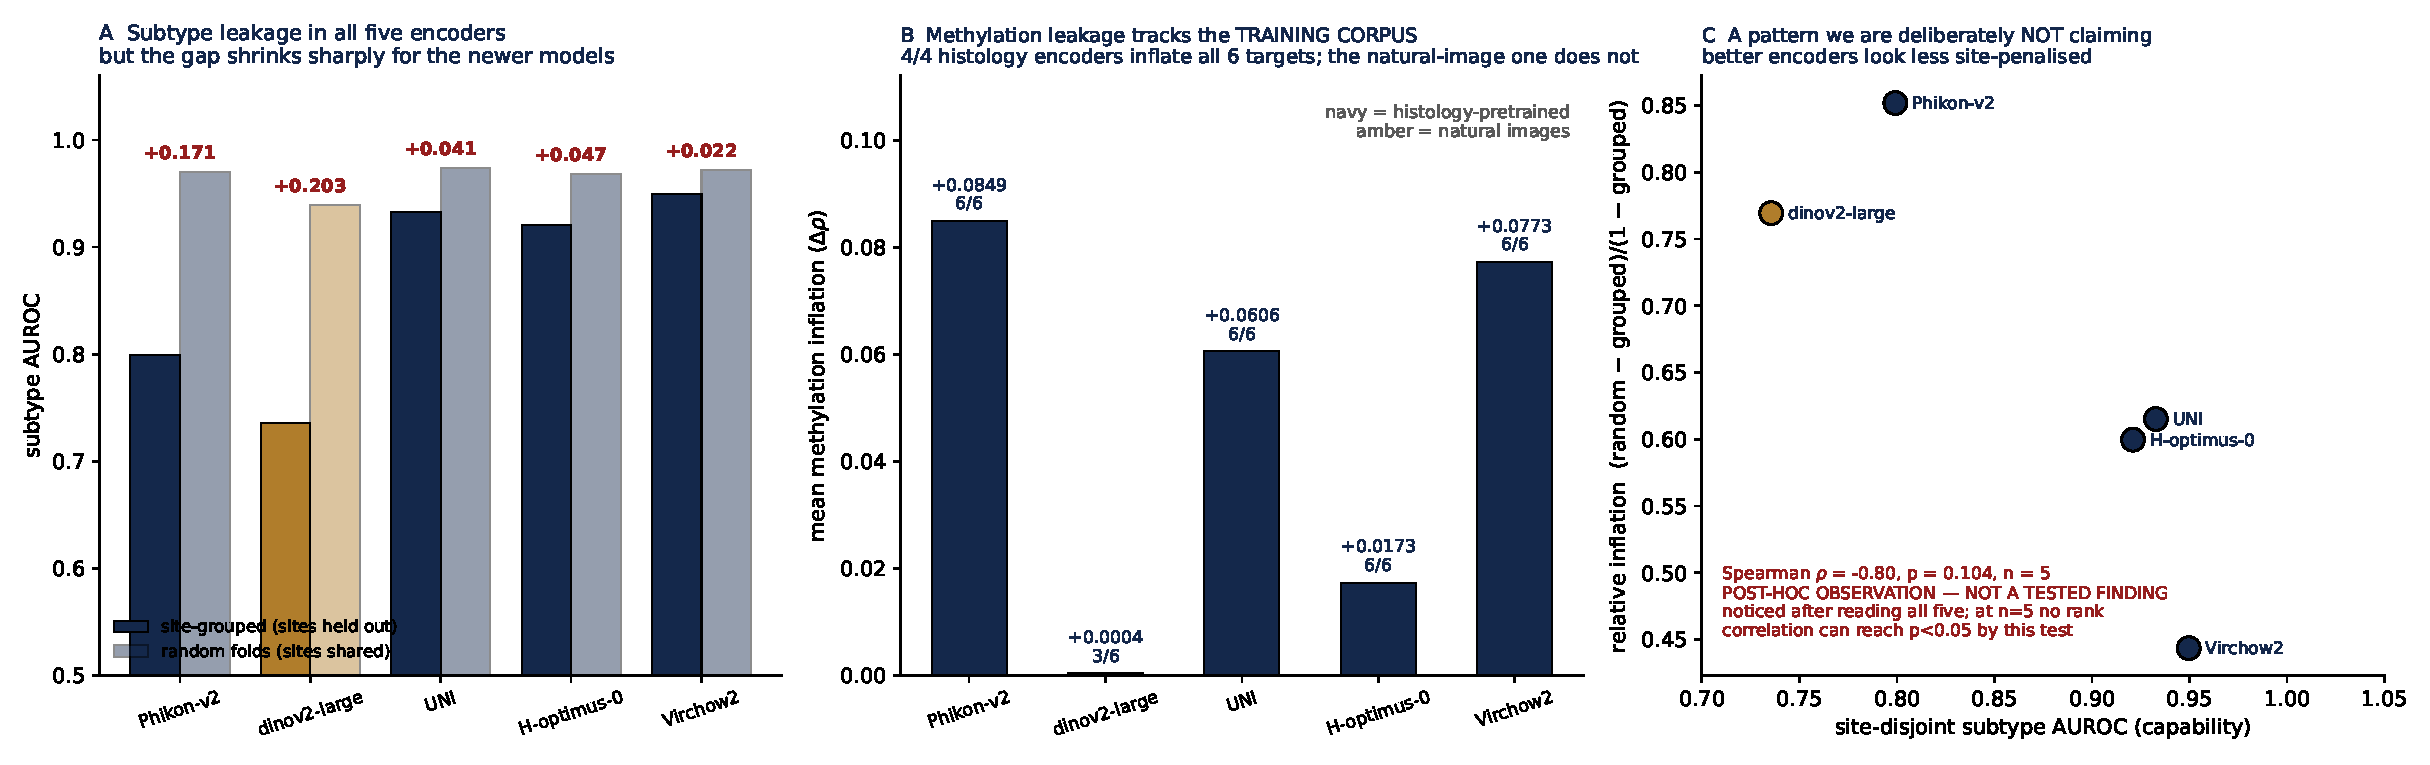
\includegraphics[width=\textwidth]{r21_panels.pdf}
\end{center}
\noindent{\small\color{qgrey}\textbf{A} Subtype, both fold regimes. \textbf{B} Methylation
inflation coloured by training corpus. \textbf{C} A post-hoc pattern, labelled as one.}

\subsection{Per-target methylation inflation}

\begin{center}
\small
\begin{tabular}{@{}lrrrrr@{}}
\toprule
\textbf{Target} & \textbf{Phikon-v2} & \textbf{dinov2-large} & \textbf{UNI} & \textbf{H-optimus-0} & \textbf{Virchow2} \\
\midrule
KEAP1 sig. & +0.0755 & -0.0158 & +0.0804 & +0.0207 & +0.0818 \\
global & +0.0783 & -0.0145 & +0.0586 & +0.0170 & +0.0750 \\
island & +0.1176 & +0.0418 & +0.0532 & +0.0056 & +0.0747 \\
open sea & +0.0610 & +0.0003 & +0.0573 & +0.0169 & +0.0704 \\
TSS200 & +0.1184 & +0.0048 & +0.0596 & +0.0294 & +0.0893 \\
gene body & +0.0589 & -0.0144 & +0.0545 & +0.0145 & +0.0727 \\
\bottomrule
\end{tabular}
\end{center}

\noindent Only \texttt{dinov2-large} has targets moving the wrong way. Every histology encoder is
positive on all six, which is what makes the corpus split legible rather than a difference of degree.

\section{Subtype leakage is universal but not constant}

The relative figure runs from 0.4435 to
0.8518, and site-disjoint capability from
0.7356 to
0.9497. The three newer pathology models are far
better at the site-disjoint task than Phikon-v2 --- Virchow2 reaches
0.9497 against Phikon-v2's
0.7992 --- and show correspondingly smaller inflation.

So ``a fold-assignment artefact of +0.1710'' is a statement about a
particular encoder in 2024, not a constant of the archive. The leakage is real in every encoder
tested; its size is not transferable.

\section{A pattern we are deliberately not claiming}

Panel C plots relative inflation against site-disjoint capability. It looks like a clean inverse
relationship: Spearman $\rho = -0.80$, $p = 0.104$,
$n = 5$.

\textbf{We are not reporting that as a finding, and the config says so.} It was noticed
\emph{after} all five encoders were read. Testing a hypothesis on the data that suggested it is
the precise move this programme exists to police, and at $n = 5$ no rank
correlation can reach $p<0.05$ by this test regardless of how clean the picture looks. What it
licenses is a pre-registration --- fix the rule, then test it on encoders not used here --- not a
conclusion. It is recorded in \texttt{results.json} under
\texttt{post\_hoc\_observation} with \texttt{STATUS} set accordingly.

\section{Controls}

The Phikon-v2 arms were re-run through the same harness and still match R15: subtype
0.7992 / 0.9703, KEAP1
0.6642, mean methylation inflation
0.0849. All gates in \texttt{evidence/gates.json} passed. Every
arm covers the same 760 patients and 67 sites.

KEAP1 inflation stays small in all five (+0.0018 to
+0.0436), which is what R15 predicted on the mechanistic
grounds that mutation status has no institutional prevalence structure to exploit. A prediction made
for a reason, holding across five encoders chosen for other reasons, is worth more than the same
number from one.

\section{Limitations}

\textbf{Five encoders, one archive, one cohort.} TCGA lung, 760 patients, 67 sites, the same
slides and the same tiles throughout.

\textbf{Corpus is confounded with vintage and capacity.} The three pathology models are newer,
larger and trained on more data than Phikon-v2, and dinov2-large differs in corpus \emph{and} in
being the only non-pathology model. A corpus-level statement is the most parsimonious reading of
Panel B, not the only possible one.

\textbf{Normalisation is not held constant.} H-optimus-0 prescribes its own; forcing ImageNet
statistics on it would have crippled it. Each model gets its own preprocessing, which is correct
practice and a departure from R18's tighter design.

\textbf{CLS-only readout.} Virchow2's authors recommend concatenating the class token with the
mean of the patch tokens. Holding the readout constant is what makes five encoders comparable, but
it may understate Virchow2's absolute capability.

\textbf{Two of the five are non-commercially licensed.} UNI and Virchow2 are CC-BY-NC-ND-4.0;
Phikon-v2, dinov2-large and H-optimus-0 are not. Each arm records its encoder's licence in the
feature files. Anything that could read as commercial should rest on the Apache-2.0 arm.

\section*{Reproducing this report}

\texttt{evidence/encode\_pathfm.py} (the three encoders, pinned),
\texttt{evidence/mil\_encoder\_compare.py} (the twenty arms),
\texttt{evidence/m18\_five\_encoder\_survey.py} (this analysis),
\texttt{evidence/config.yaml} (SHA-256 \texttt{b23ba9307a6081c4\ldots}),
\texttt{evidence/gates.json}, \texttt{evidence/results.json},
\texttt{evidence/arms/} (all twenty raw arm JSONs).
This document: \texttt{python3 make\_report.py}. Figure: \texttt{python3 make\_figure.py}.

\end{document}
